\section{Генерация текстовых задач}

В Первом разделе представлены работы, связанные Текстовыми задачами. 
%Работа велась на языке \texttt{JavaScript}, с использованием вспомогательных функций для визуализации и генерации условий.
Так как в 
%15, 21 "текстовые задачи"
%рассказать про декорации, про chislitlx(пулл реквест с r2), сочетания 
%предварительные сведения (функции, кратко ,генассерт и тп)
%платформа час-ЕГЭ (то что сделала сама "хвалюсь") для "реализации задачи мною были разработаны" и тп, 
% то что существует - описываю как факт (а.к.а предварительные сведения)
% 4 1)отдельно (формулы) естественно появляется обратная задача. 2)Сослаться на Латех (MathJax) основные команды которыми пользуемся в Латехе texfrag и тп 
%7 делится на две главы. Задача с чертежом коорд.оси (предвор сведения, разработанные библ функции, шаблоны)
% вторая - задача на сравнение чисел (как устроено округление,autoLateX )
% в заключении написать количество вып задач по категориям 
%в данной главе (тото это тамто и тп)
% не менее 10 шаблонов сумарно затронув каждую категорию 
% где-то 45-50 страниц....
% про расвнение чисел очень долго целых чисел не было, все числа были дробные, 0.1+0.2!=0.3 надо быть осторожным и тп расскажи!! 
%захожу в калатог, через меню переключаемся на тест на печать внимательно (?) выставить нулями все задания кроме того что нужно ставить галочку " экспорт в латех" 
%ставим запуск,жду,думаю, падает зипка с задачами в латехе, в перемешку 
%исходная задача/код/полученная задача (сгенерин текст)
При построении текстовых шаблонов задач важно обеспечить как вариативность формулировок, так и корректность числовых и языковых выражений. Для этого в проекте применяются следующие инструменты.

\subsection{Декорации}

Чтобы увеличить количество уникальных вариантов задач, сохраняя их математическую суть, используются так называемые ``декорации''~--- элементы окружения, которые можно менять без потери смысла задачи: имена персонажей, место действия, цель, контекст. 
Для этого создаются массивы строк, а функция \texttt{iz()} случайным образом выбирает элемент из массива.

Пример:
\begin{lstlisting}
let contract = ['о дружбе', 'во избежание двойного налогообложения',
    'о безвизовом режиме', 'об экологической среде',
    'по гуманитарным вопросам', 'по вопросам безопасности'].iz();
\end{lstlisting}
\textsl{Задача №514913.}
\lstinputlisting[]{code/21/514913.js} 

Если необходимо выбрать два случайных, но не повторяющихся элемента, используется форма \texttt{iz(2)}:  
\begin{lstlisting}
let tapeName = sklonlxkand(['лента', 'верёвка', 'нитка'].iz(2));
\end{lstlisting}
\textsl{Задача №2434.}
%добавить пример до/после 
\lstinputlisting[]{code/21/2434.js} 
До:
После:

\includegraphics[width=1.4\textwidth]{2434-21-1.png}

\includegraphics[width=1.4\textwidth]{2434-21-2.png}

Чтобы каждый раз не задавать список декораций,у нас есть несколько заготовленных, которые используются от задаче к задаче. Например \texttt{om.meltov={}} и они могут быть рассписаны даже по нескольким падежам.

Например: 
\begin{lstlisting}
om.meltov={}
om.meltov.ie = ['фонарик', 'флакон шампуня', 'флэшка', 'компакт-диск', 'сувенир', 'матрёшка', 'магнит на холодильник', 'сборник тестов для подготовки к ЕГЭ', 'тетрадь', 'учебник', 'цветочный горшок'];
\end{lstlisting}
В задаче же благодаря этому можно записать короче:
\begin{lstlisting}
let item = sklonlxkand((om.meltov.ie).iz());
\end{lstlisting}
\textsl{Задача №314120.}

Как вы могли заметить, некоторые декорации являются словосочетанием, например "флакон шампуня", "цветочный горшок", "магнит на холодильник" и так далее. И для более коректной работы \texttt{.ie} и других падежей у нас есть словарь \texttt{lxsoch.js}
Однако недавно было выявленно, что если рядом со словосочетанием стоит число, то оно должно изменяться. например "3 цветочных горшка" или " 4 флакона шампуня". Они очень схожи с родительным падежом множественного числа, но отличаются. Так что мною был добавлен в  
\texttt{lxsoch.js} \texttt{.r2}. Это падеж, в котором учтено изменения слова из-за числительного. 
%добавить пример Саши?

\subsection{Склонения сушествительных}

В силу особенностей русского языка слова должны корректно изменяться по падежам и числам. Для этого применяется функция \texttt{sklonlxkand}, позволяющая генерировать правильные словоформы.  
После выбора слова к нему можно обратиться по падежу и числу. Например, \texttt{.ie} означает именительный падеж, единственное число.  

Пример использования:
\begin{lstlisting}
let typeOfFlowerInVases =
  sklonlxkand(['роза','гвоздника','ромашка','лилия',
               'мак','ирис','лаванда','мимоза'].iz());
NAtask.setTask({
  text: 'На прилавке цветочного магазина стоят три вазы с '
    + typeOfFlowerInVases.tm + ': ' + vaseColor[0] + 'ая, '
    + vaseColor[1] + 'ая, ' + vaseColor[2] + 'ая.' 
    + ' Слева от ' + vaseColor[2] + 'ой вазы '
    + chislitlx(leftOfThirdVase, typeOfFlowerInVases, '$')
    + ', справа от ' + vaseColor[0] + 'ой вазы '
    + chislitlx(righttOfFirstVase, typeOfFlowerInVases, '$') + '. '
    + 'Всего в вазах '
    + chislitlx(allFlowerInVases, typeOfFlowerInVases, '$') + '. '
    + 'Сколько ' + typeOfFlowerInVases.rm + ' в '
    + vaseColor[1] + 'ой вазе?',
  answers: secondVaseCountFlower,
});
\end{lstlisting}
\textsl{Задача №515842.}

\lstinputlisting[]{code/21/515842.js} 
До:
После:

\includegraphics[width=1\textwidth]{515842-21.png}    

Для корректного согласования числительных с существительными используется функция \texttt{chislitlx}. Она автоматически выбирает нужную форму слова в зависимости от числа.  
% написать про ceil() 
%добавить примеры до/после
Пример:
\begin{lstlisting}
let numberOfApartamentPerFloor = sluchch(3, 12, 1);
NAtask.setTask({
  text: 'В доме, в котором живет ' + nameOfPerson + ', ' +
    '$' + floorNumber + '$ этажей и несколько подъездов. На каждом этаже находится по ' +
    chislitlx(numberOfApartamentPerFloor, 'квартира', '$') + '. '
    + nameOfPerson + ' живет в квартире №' + '$' + apartamentNumber + '$' + '. '
    + 'В каком подъезде живет ' + nameOfPerson + '? ',
  answers: '$' + (apartamentNumber /
             (floorNumber * numberOfApartamentPerFloor)).ceil() + '$',
});
\end{lstlisting}
\textsl{Задача №77351.}

\subsection{Проверка условий (генерация утверждений)}

Помни во всех шаблонах вы так или иначе увидете окружение \texttt{retryWhileError}, которое ограничевает количество перезапусков, плюсом ещё и фиксирует какие проверки не были пройдены и выводить их на экран. Само собой ошибки видны только разработчикам Во время отладки.
\function{retryWhileError}{theFunction, maxIterations,maxCollectedErrors}

Пример: 
\lstinputlisting[]{code/15/509768.js}
До: 
После: 

\includegraphics[width=1\textwidth]{509768-15-1.png}  

\includegraphics[width=1\textwidth]{509768-15-2.png}  

Для контроля корректности задачи применяются функции \texttt{genAssert} и её вариации. Принцип работы:  
\begin{itemize}
    \item если условие не выполнено~--- фиксируется ошибка;
    \item шаблон перезапускается;
    \item если достигнуто максимальное количество перезапусков, выводятся накопившиеся ошибки с указанием количества.
\end{itemize}

Пример использования:
\begin{lstlisting}
let students = sl(200, 10000, 10);
let percent = sl(10, 90, 1); 
genAssert(students.kratno(100 / percent),
          "количество учащихся не кратно 100/процент");
\end{lstlisting}
\textsl{Задача №77340.}

Также часто используется функция \function{genAssertZ1000}{number, message}, проверяющая точность чисел: если у числа более трёх знаков после запятой, шаблон перезапускается.  
\function{genAssertIrreducible}{numerator, denominator, message} - проверка на несократимость дроби.

Пример:
\begin{lstlisting}
let prise = sl(100, 2000, 10);
let percentSecondMonth = sl(10, 90, 1);
let percentThirdMonth = sl(10, 90, 1);

let middlePrise = prise * (1 + [1, -1][randFirst] * 0.01 * percentSecondMonth);
let finalePrise = middlePrise * (1 + [1, -1][randSecond] * 0.01 * percentThirdMonth);

genAssertZ1000(finalePrise / 10,
               'Число имеет более 2 знаков после запятой');
\end{lstlisting}
\textsl{Задача №77349.}

\lstinputlisting[]{code/15/77349.js}
До:
После:

\includegraphics[width=1\textwidth]{77349-15-1.png}
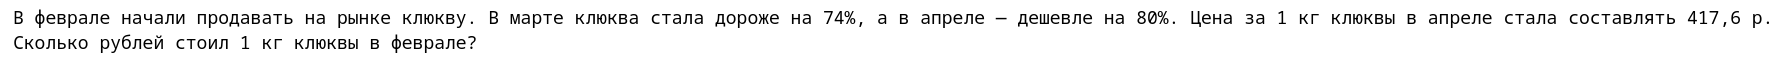
\includegraphics[width=1\textwidth]{77349-15-2.png}

В некоторых случаях может применяться \texttt{slKrome} ,он работает как \texttt{sluchch} - создает случайное число. Однако с условием что оно  отличное от
		первого параметра (первый параметр может быть числом, строкой, массивом или функцией),
		второй и третий параметры - это диапазон генерации, а четвертый параметр - шаг (по умолчанию это 1).
Пример:
\begin{lstlisting}
let mlnRuble = slKrome([100], 10, 200, 1);
\end{lstlisting}
\textsl{Задача №506346.}

\texttt{kratno} является функцией, провищяющее кратно ли данное число другому. Чаще всего используем в genAssert для проверки
Пример:
let students = sl(200, 10000, 10);
let percent = sl(10, 90, 1);
genAssert(students.kratno(100 / percent), "количество учащихся не кратко 100/процент");
\textsl{Задача №77340.}

\texttt{NAtask.modifiers.allDecimalsToStandard} мы используем в случаях работы с десятичными числами и дробями, для более коррктеного расчёта java script формул.
 Это помогает избежать излишней точности.

Пример:
\begin{lstlisting}
 let difference = sl(2, 20, 1);
        let minAngle = (360 / (2 * difference + 1));
        let maxAngle = (360 / (difference + 2));

        let result = maxAngle.floor() - minAngle.floor() - Number(maxAngle % 1 == 0 || minAngle % 1 == 0);

        NAtask.setTask({
            text: 'Три луча, выходящие из одной точки, разбивают плоскость на $3$ ' +
                'разных угла, измеряемых целым числом градусов. Наи' + moreOrLess + 'ьший угол в ' +
                chislitlx(difference, 'раз', 'v$') + ' ' + moreThanLessThan +
                ' наи' + lessOrMore + 'ьшего. Сколько значений может принимать величина среднего угла?',
            answers: result,
        });
        NAtask.modifiers.allDecimalsToStandard();
\end{lstlisting}       
\textsl{Задача №514918.}

\lstinputlisting[]{code/21/514918.js}
До:
После:

\includegraphics[width=1\textwidth]{514918-21.png}

\subsection{Разнообразие в текстовых задачах}
%не забудь вставить картинки(до и после) для каждого условия этих задачек
И самое главное для текстовых задач, возможность их разнообразить. Дело в том что изначально даётся достаочно много условий в задаче,от чего можно написать альтернативные варианты задачи. Что помогает ученикам лучше запонимать не просто последовательность решения, а принцип.
Чаще всего от изменений условия задачи на альтернативное сильно меняется и текст, по этому мы используем questions. Он позволяется разбить на несколько заданий одно и для каждого приписать свой ответ. Если же у них общее начало то можно записать его в первый text, а если одинавокое окончение то 
дописать его в postquestion.

Пример1: 
\lstinputlisting[]{code/15/506426.js} 
\textsl{Задача №506426.}
До:
После:

\includegraphics[width=1\textwidth]{506426-15-1.png}

\includegraphics[width=1\textwidth]{506426-15-2.png}

\includegraphics[width=1\textwidth]{506426-15-3.png}

Пример2:
\lstinputlisting[]{code/15/522673.js} 
\textsl{Задача №522673.}
До:
После:

\includegraphics[width=1\textwidth]{522673-15-1.png}

\includegraphics[width=1\textwidth]{522673-15-2.png}

\includegraphics[width=1\textwidth]{522673-15-3.png}

\includegraphics[width=1\textwidth]{522673-15-4.png}

\includegraphics[width=1\textwidth]{522673-15-5.png}

\includegraphics[width=1\textwidth]{522673-15-6.png}